\documentclass{article}
\usepackage{graphicx} % Required for inserting images
\usepackage{listings}
\usepackage{xcolor}
\usepackage{forest} %p Per disegnare grafi

\colorlet{punct}{red!60!black}
\definecolor{background}{HTML}{EEEEEE}
\definecolor{delim}{RGB}{20,105,176}
\colorlet{numb}{magenta!60!black}

\lstdefinelanguage{json}{
    basicstyle=\normalfont\ttfamily,
    numbers=left,
    numberstyle=\scriptsize,
    stepnumber=1,
    numbersep=8pt,
    showstringspaces=false,
    breaklines=true,
    frame=lines,
    backgroundcolor=\color{background},
    literate=
     *{0}{{{\color{numb}0}}}{1}
      {1}{{{\color{numb}1}}}{1}
      {2}{{{\color{numb}2}}}{1}
      {3}{{{\color{numb}3}}}{1}
      {4}{{{\color{numb}4}}}{1}
      {5}{{{\color{numb}5}}}{1}
      {6}{{{\color{numb}6}}}{1}
      {7}{{{\color{numb}7}}}{1}
      {8}{{{\color{numb}8}}}{1}
      {9}{{{\color{numb}9}}}{1}
      {:}{{{\color{punct}{:}}}}{1}
      {,}{{{\color{punct}{,}}}}{1}
      {\{}{{{\color{delim}{\{}}}}{1}
      {\}}{{{\color{delim}{\}}}}}{1}
      {[}{{{\color{delim}{[}}}}{1}
      {]}{{{\color{delim}{]}}}}{1},
}

\title{Università degli studi di Modena e Reggio Emilia\\
        Dipartimento di ingegneria "Enzo Ferrari"}

%\author{ALESSANDRO APPIO}
\date{2024}

\begin{document}

\lstset{
    basicstyle=\ttfamily,
    keywordstyle=\color{blue},
    stringstyle=\color{orange},
    commentstyle=\color{green},
    showstringspaces=false,
    breaklines=true,
    frame=single
}
\lstset{
    language=C++,                     % Linguaggio del codice
    backgroundcolor=\color{background},
    basicstyle=\ttfamily\small,       % Stile del font
    keywordstyle=\color{blue},        % Colore delle keyword
    stringstyle=\color{orange},       % Colore delle stringhe
    commentstyle=\color{green},       % Colore dei commenti
    showstringspaces=false,           % Non mostra gli spazi nelle stringhe
    numbers=left,                     % Numerazione delle righe a sinistra
    numberstyle=\tiny\color{gray},    % Stile della numerazione
    stepnumber=1,                     % Ogni riga numerata
    breaklines=true,                  % A capo automatico delle righe lunghe
    frame=single,                     % Cornice attorno al codice
    captionpos=b,                     % Posizione del titolo: b (bottom)
}

\maketitle

\bigskip
\hrule
\bigskip

\begin{center}
  \noindent\huge{Controllo remoto e setup di un mezzo terrestre}
\end{center}

\bigskip
\hrule
\bigskip

\vfill
\begin{center}
  \large{\textbf{Relatore:} Paolo Burgio}\\
  \large{\textbf{Candidato:} Alessandro Appio}\\
  \bigskip
  \large{Anno accademico: 2023/2024}
\end{center}

\newpage
\tableofcontents
\newpage

\newpage
\section{Introduzione} \label{introduzione}
\subsection{Guida remota e guida autonoma}
La guida autonoma e la guida remota sono due tecnologie che promettono di trasformare radicalmente il modo in cui ci muoviamo, rendendo i trasporti più sicuri, efficienti e sostenibili, e stanno al centro di una rivoluzione tecnologica: la mobilità intelligente.

\noindent La guida autonoma rappresenta un complesso sistema tecnologico che integra una serie di avanzate tecnologie, metodologie e tecniche finalizzate a consentire il movimento di un veicolo senza necessità di intervento umano diretto. Un veicolo autonomo è infatti dotato della capacità di analizzare l'ambiente circostante, elaborare un percorso ottimale in base ai dati raccolti, e seguire tale percorso in modo autonomo. 

\noindent Secondo la Society of Automotive Engineers international (SAE)\cite{SAE_autonomous_vehicle} il concetto di guida autonoma si può dividere in 6 livelli:

\begin{itemize}
  \item Livello 0: Il veicolo non ha capacità di guida autonoma e tutta la responsabilità è conferita al guidatore  
  \item Livello 1: Il veicolo assiste il guidatore in maniera limitata, agendo su acceleratore, freno e sterzo. La responsabilità rimane però completamente nelle mani dell'umano 
  \item Livello 2: Il veicolo ha le capacità di controllare simultaneamente la direzione, l'accelerazione e la frenata, ma il guidatore deve sempre e comunque rimanere vigile e monitorare le scelte prese dal veicolo
  \item Livello 3: Il veicolo può prendere completamente il controllo della guida ma solo in determinate situazioni (e.g. in autostrada) e il conducente deve essere pronto a prendere il controllo quando richiesto dal sistema
  \item Livello 4: Il veicolo può gestire tutte le funzioni di guida in maniera autonoma in quasi tutte le condizioni, ma può comunque richiedere l'intervento umano in situazioni straordinarie (e.g. zone non mappate)
  \item Livello 5: Il veicolo è completamente autonomo e non necessita di intervento umano
\end{itemize}

\noindent I processi fondamentali della guida autonoma vengono generalmente suddivisi in tre fasi distinte: percezione (perception), pianificazione (planning) e controllo (control).
La percezione riguarda la capacità del veicolo di raccogliere informazioni dall'ambiente circostante attraverso sensori avanzati, che possono includere telecamere, radar, Lidar e altre tecnologie di rilevamento. Questi dati vengono poi elaborati nella fase di pianificazione, durante la quale il sistema valuta le possibili traiettorie e sceglie il percorso più sicuro ed efficiente da seguire. Infine, la fase di controllo si occupa dell'esecuzione del movimento del veicolo lungo il percorso stabilito, garantendo che vengano seguite le decisioni prese nella fase di pianificazione.

\begin{figure}[H]
  \centering
  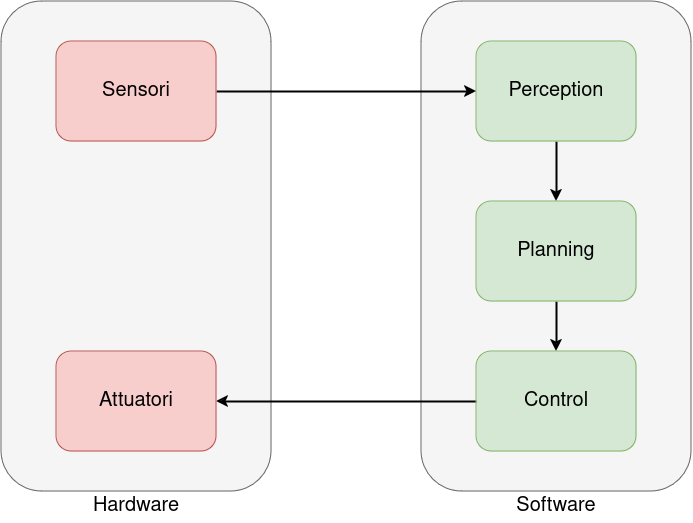
\includegraphics[width=1\textwidth]{figures/guida_autonoma.png}
  \caption{Semplice stack di guida autonoma}
  \label{guida_autonoma}
\end{figure}

\noindent Se nella guida autonoma le decisioni vengono elaborate da un sistema informatico a bordo del veicolo, il concetto di guida remota si riferisce a un tipo di guida in cui le decisioni relative alla direzione e al movimento del veicolo vengono elaborate in remoto. A seconda della strategia con la quale vengono prese queste decisioni, la guida remota si suddivide in:

\begin{itemize}
    \item Driver: le decisioni relative alla direzione e al movimento del veicolo vengono prese da un operatore umano che opera a distanza, capace di osservare i dati rilevati dai sensori presenti a bordo del mezzo
    \item Driverless: le decisioni vengono prese da uno stack di guida autonoma eseguito da un server remoto che prende in input i dati rilevati dai sensori presenti a bordo del mezzo e trasmette al veicolo istruzioni puntuali sul movimento da compiere 
\end{itemize}

\noindent La guida remota opera utilizzando tecnologie quali sensori, attuatori, e reti di comunicazione. In questo scenario, la logica che impartisce ordini non si trova fisicamente all'interno del veicolo, ma interagisce con esso attraverso un'interfaccia remota, sfruttando la trasmissione dei dati in tempo reale per monitorarlo e controllarlo. Tale approccio rende possibile la guida di veicoli in situazioni in cui la presenza fisica del conducente potrebbe non essere necessaria o praticabile

\subsection{Tecnologie IOT}
L'avvento dell'Internet of Things (IoT) ha inaugurato una nuova era tecnologica, caratterizzata dalla connettività pervasiva e dall'intelligenza distribuita. Questa rivoluzione digitale sta trasformando profondamente numerosi settori, tra cui la logistica. La crescente complessità delle catene di approvvigionamento globali, unita alla crescente domanda di efficienza e tracciabilità, rende l'IoT una tecnologia sempre più strategica per le aziende del settore.

\noindent L'IoT è un concetto che descrive una rete di dispositivi fisici connessi tra loro attraverso Internet, che sono capaci di scambiare dati e di comunicare con altri dispositivi, sistemi e/o servizi. Questi dispositivi, che possono includere sensori, elettrodomestici, veicoli (come nel nostro caso), sistemi di sicurezza, macchinari industriali e molto altro, sono dotati di sensori, software e altre tecnologie che permettono loro di raccogliere e condividere dati in tempo reale.

\noindent La guida remota, ovvero la possibilità di controllare un veicolo a distanza attraverso una connessione di rete, rappresenta una delle applicazioni più promettenti dell'IoT nel settore dei trasporti.

\subsection{Scopo della tesi}
L'obiettivo principale di questa tesi è quello di sviluppare un sistema di guida capace di operare sia in modo autonomo che in modalità di guida remota.

\noindent Si consideri lo scenario in cui il veicolo e l'hardware a bordo siano intatti e che il conducente sia sempre vigile, controllando il comportamento del mezzo anche in caso di errore o malfunzionamento. Su richiesta del conducente, il sistema potrà operare in questo caso in modalità autonoma.

\noindent Supponiamo ora che il guidatore non sia nelle sue condizioni ottimali e che, per esempio, a causa di un malore, non possa rimanere vigile e controllare adeguamente il veicolo. In questo caso, un ente terzo sarà in grado collegarsi al veicolo, passare alla modalità remota e mettere in sicurezza l'operatore conducendolo eventualemte all'ospedale più vicino.

\noindent Questo approccio duale consente al veicolo di navigare in modo completamente indipendente quando le circostanze lo permettono, utilizzando tecnologie di percezione, pianificazione e controllo integrate, ma offre al contempo la flessibilità di essere controllato a distanza da un operatore umano o da uno stack di guida autonoma qualora la situazione lo richieda. La possibilità di commutare tra guida autonoma e remota mira a garantire la massima sicurezza, adattabilità e versatilità del veicolo in una varietà di scenari operativi.


\newpage
\section{Piattaforma di sviluppo}
In questa sezione si descrive come è composta e come è stata assemblata la piattaforma per lo sviluppo e il testing.

\subsection{Rover AgileX}
Il veicolo selezionato per lo sviluppo della presente tesi è un rover terrestre prodotto da AgileX, modello Hunter. Questo rover è dotato di 3 motori elettrici (2 per la trazione posteriore ed 1 per lo sterzo), di sensori dediti all'analisi del movimento delle ruote e di una board dedicata al controllo dei motori e all'interfacciamento del mezzo con un calcolatore esterno. L'intera scocca è realizzata in alluminio rendendolo molto resistente ma allo stesso tempo non eccessivamente pesante.

\begin{figure}[H]
  \centering
  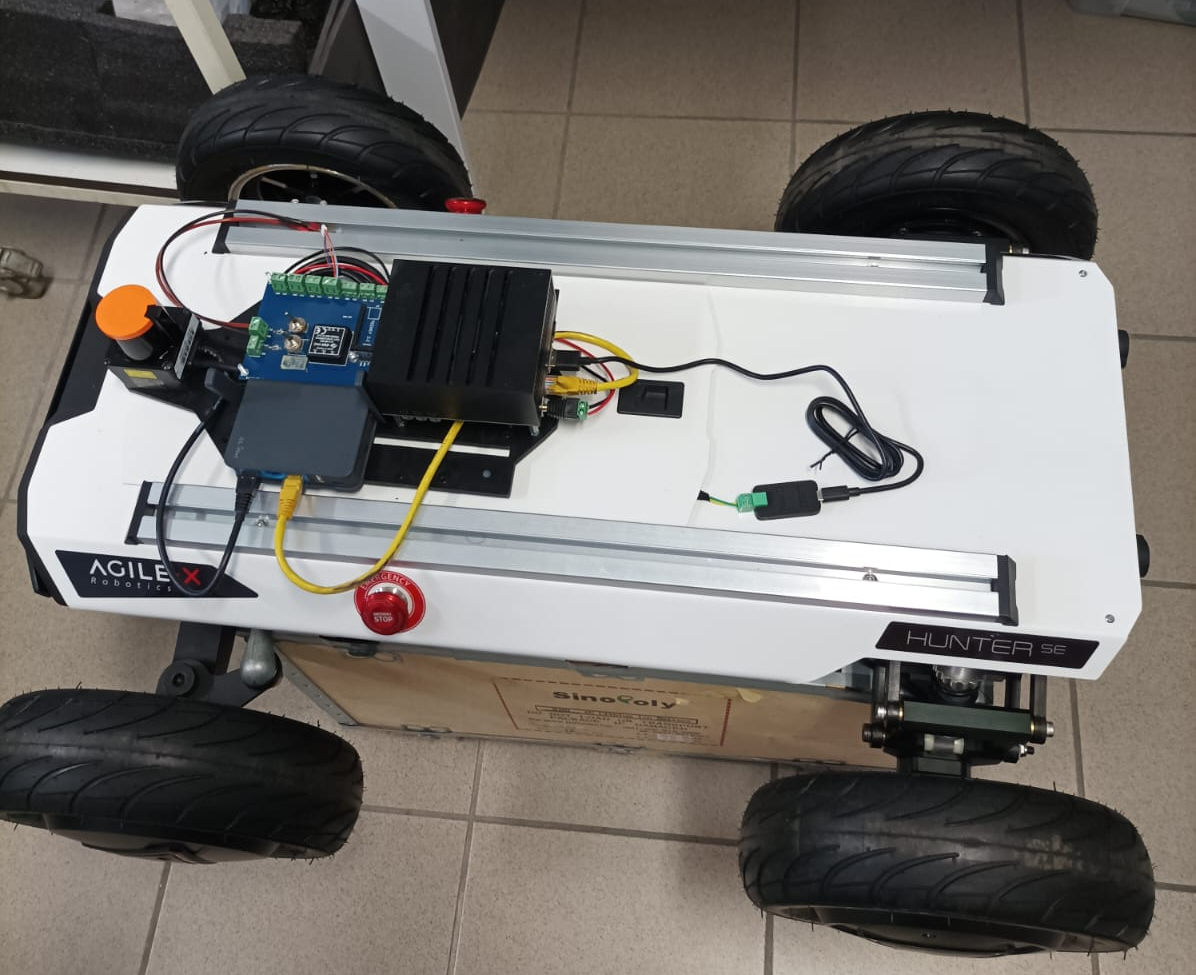
\includegraphics[width=0.8\textwidth]{figures/franco.png}
  \caption{Rover assemblato}
  \label{Rover assemblato}
\end{figure}

\noindent La scheda di controllo del rover è collegata alla porta usb del computer embedded tramite un'apposita periferica e consente una comunicazione efficiente e affidabile. Il modello Hunter è stato scelto per le sue avanzate caratteristiche tecniche e per la sua versatilità, che lo rendono particolarmente adatto alle esigenze del progetto.

\noindent Oltre a fornire un'interfaccia per il controllo diretto, il veicolo è in grado di raccogliere e trasmettere una serie di dati diagnostici e operativi fondamentali per il monitoraggio e l'analisi delle sue prestazioni. Tra questi dati, un ruolo cruciale è ricoperto dall'odometria. 

\noindent L'odometria è una misura che permettte la stima dello spostamento di un veicolo a partire dallo spostamento delle ruote, ed è essenziale per la navigazione e la stima della posizione del rover, poiché permette di determinare il percorso seguito dal veicolo e la distanza percorsa. Questi dati, insieme ad altre informazioni sullo stato del veicolo, contribuiscono a garantire un controllo preciso e ad alimentare i sistemi di guida autonoma e remota previsti dal progetto.

\subsubsection{Protocollo CAN}
La scheda di controllo del rover è basata sul protocollo Controller Area Network (CAN), un protocollo seriale molto versatile sviluppato dall'azienda Bosh nel 1993 e molto utilizzato in ambito automotive e automazione industriale. Questa interfaccia seriale è accessibile tramite 2 segnali denominati CAN-HIGH e CAN-LOW, collegati ad una periferica USB interfacciata al computer di bordo.

\noindent Il protocollo CAN è utilizzato in quanto è un protocollo molto resistente alle interferenze (grazie a una tecnica di bit dominante e recessivo), veloce e per niente costoso.  

\subsection{GPGPU}
Un elemento cruciale per la realizzazione di questa tesi è stato l'identificazione e la selezione di un calcolatore embedded che possa comunicare con i sensori e il rover e che possa gestire il carico di tutti gli algoritmi e i processi necessari per la guida autonoma.

\noindent La scelta è ricaduta su una scheda di casa Nvidia, modello AGX Jetson Xavier, una  General Purpose Graphic Processing Unit (GPGPU). Questa scelta è motivata dall'elevata capacità di elaborazione parallela che solo una GPGPU può fornire, capacità che risulta particolarmente vantaggiosa per l'esecuzione di complessi algoritmi di percezione, pianificazione e controllo, da svolgere in tempo reale. La GPGPU selezionata opera con il sistema operativo Ubuntu 20.04 Focal Fossa, noto per la sua stabilità e compatibilità con l'hardware scelto.

\begin{figure}[H]
  \centering
  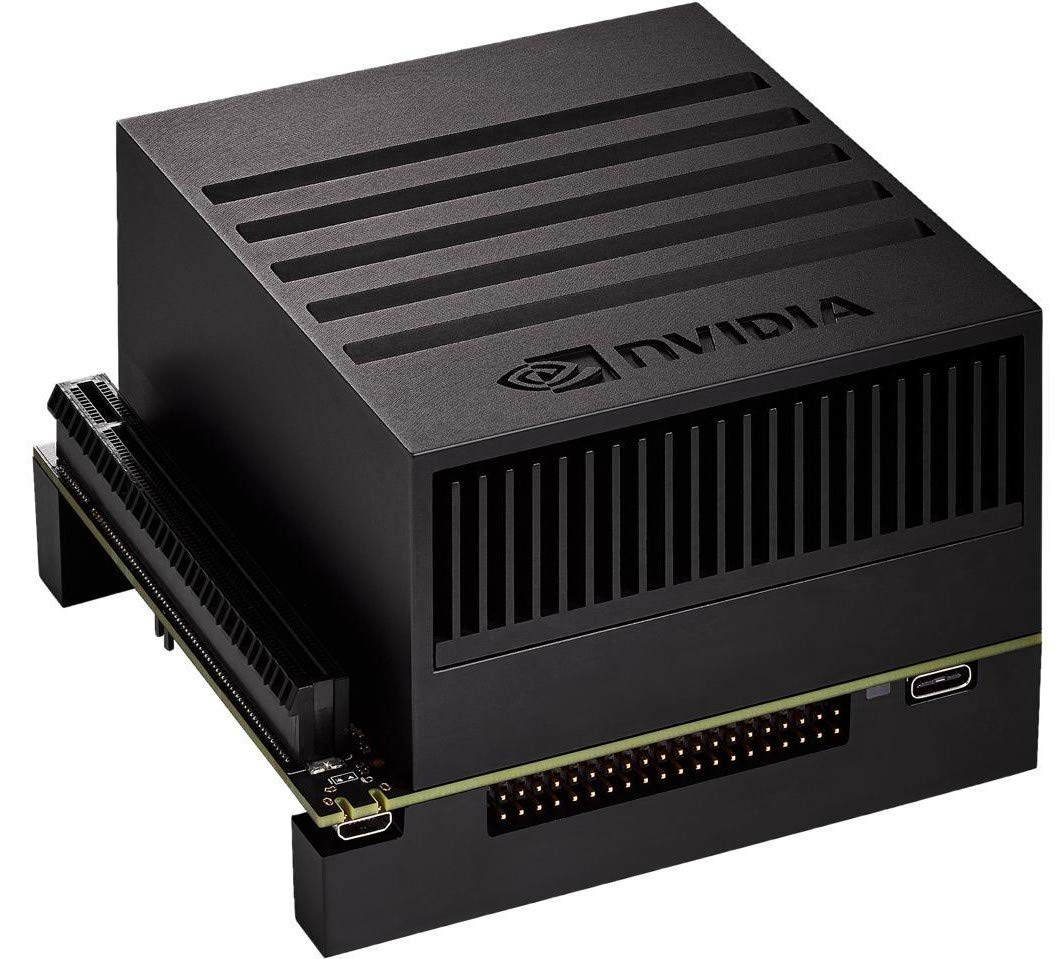
\includegraphics[width=0.8\textwidth]{figures/xavier.jpg}
  \caption{Nvidia AGX Jetson Xavier}
  \label{Nvidia AGX Jetson Xavier}
\end{figure}

\noindent Di seguito una tabella riassuntiva delle principali caratteristiche della GPGPU Utilizzata:

\begin{center}
  \begin{table}[H]
  \centering
    \begin{tabular}{|c|c|}
      \hline 
      GPU& GPU con architettura NVIDIA Volta a 512 core con 64 Tensor Core \\
      \hline 
      CPU& CPU NVIDIA Carmel Arm® v8.2 8-core 64-bit 8 MB L2 + 4 MB L3 \\
      \hline 
      Memoria& LPDDR4x 32 GB 256-bit 136,5 GB/s \\
      \hline
      Storage& eMMC 5.1 32 GB espandibile con scheda di memoria e/o SSD NVMe \\ 
      \hline
      Alimentazione& 10 W - 30 W \\
      \hline
    \end{tabular}
    \caption{Specifiche tecniche della GPGPU Nvidia AGX Jetson Xavier\cite{jetson_xavier}}
  \end{table}
\end{center}

\subsection{Lidar}
Per permettere al sistema di orientarsi e navigare correttamente è necessario l'utilizzo di un sensore che permetta al veicolo di percepire l'ambiente circostante. La scelta è ricaduta su un sensore Light Detection and Ranging (LiDaR) 2D di marca Hokuio. Questo dispositivo sfrutta la tecnologia laser per determinare la distanza di vari punti nell'ambiente circostante, calcolando il tempo di ritorno dei raggi laser emessi. Il Lidar fornisce una mappa dettagliata della topografia dell'ambiente, consentendo al sistema di percezione di creare rappresentazioni, tridimensionali o bidimensionali, dello stesso e fondamentali per il riconoscimento degli ostacoli, la navigazione, la pianificazione del percorso del veicolo e la mappatura dell'ambiente circostante.

\noindent La combinazione di una GPGPU performante e un sensore Lidar avanzato rappresenta una solida base tecnologica per lo sviluppo di un sistema di guida autonoma e remota altamente efficiente.

\noindent Il sensore Lidar genera una nuvola di punti dell'ambiente circostante attraverso l'emissione di impulsi laser in un cono di 270 gradi. Ciascun punto della nuvola corrisponde alla distanza misurata tra il sensore e un elemento dell'ambiente. La distanza è determinata con accuratezza cronometrando il tempo impiegato dall'impulso laser a percorrere il tragitto andata e ritorno.

Figura \ref{Sensore Lidar} riporta un'immagine del sensore scelto.

\begin{figure}[H]
  \centering
  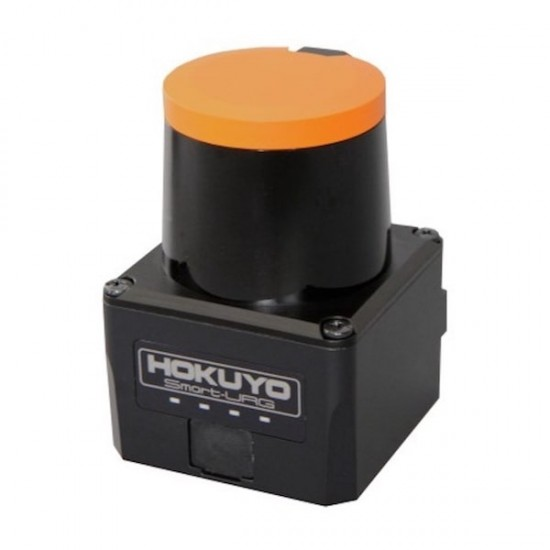
\includegraphics[width=0.8\textwidth]{figures/sensore_hokuio.jpg}
  \caption{Sensore Lidar}
  \label{Sensore Lidar}
\end{figure}

%\newpage
\subsection{Router}
In considerazione delle elevate esigenze di comunicazione proprie di un veicolo connesso, si è optato per l'integrazione a bordo di un router di rete. Tale dispositivo ha la duplice funzione di instaurare una connessione stabile e ad alta banda passante con l'infrastruttura di rete esterna, garantendo così la trasmissione fluida dei dati, e di fungere da nodo centrale per la comunicazione interna al veicolo. In particolare, il router è preposto a interconnettere il calcolatore di bordo, deputato all'elaborazione dei dati provenienti dai vari sensori, con il sensore Lidar, il quale, mediante interfaccia Ethernet, trasmette ingenti volumi di dati destinati al calcolatore. Il router scelto per il progetto è il modello GL-AR750S di marca gl.inet. Alimentato tramite porta USB direttamente sul rover, questo ruter è noto per le sue piccole dimensioni e il suo basso consumo energetico

\begin{figure}[H]
  \centering
  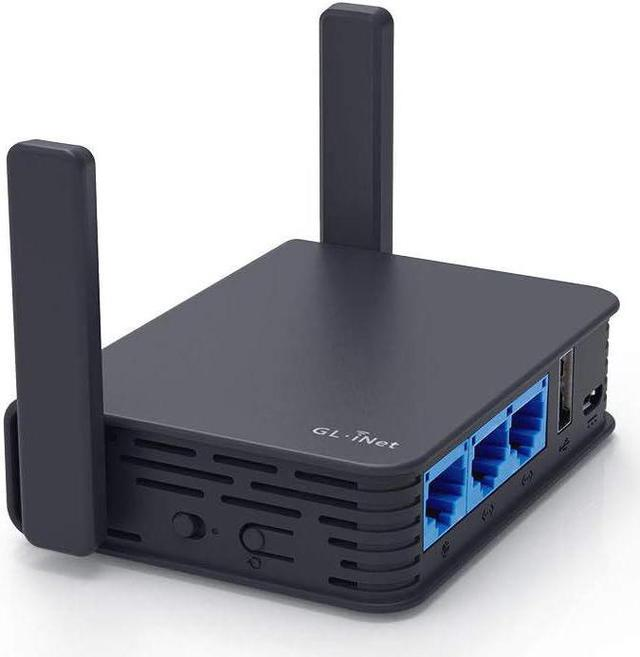
\includegraphics[width=0.8\textwidth]{figures/router.jpg}
  \caption{Router scelto per la piattaforma di sviluppo}
  \label{router}
\end{figure}


\newpage
\section{ROS}
In questa sezione si passa alla descrizione di ROS, al suo funzionamento e al suo utilizzo.
\subsection{Nodi}
Il Robotic Operating System, comunemente noto come ROS, è una piattaforma software composta da un insieme di librerie e strumenti che facilitano lo sviluppo di applicazioni dedicate al controllo e alla gestione di sistemi robotici. ROS offre un'infrastruttura flessibile e modulare che permette agli sviluppatori di creare, testare e implementare applicazioni complesse per robot in modo efficiente.

\noindent Uno degli aspetti fondamentali di ROS è la sua architettura basata su nodi, che rappresentano unità di esecuzione autonome all'interno del sistema. Un nodo può essere responsabile di una vasta gamma di funzioni, tra cui eseguire calcoli, interfacciarsi con dispositivi hardware, raccogliere dati dai sensori, e molto altro. Tuttavia, la caratteristica più distintiva di un nodo ROS è la sua capacità di comunicare in maniera integrata con altri nodi attraverso un sistema di messaggistica distribuita. Questo sistema consente ai nodi di scambiare informazioni in tempo reale, permettendo una coordinazione precisa e affidabile tra i diversi componenti di un robot.

\noindent Questa struttura modulare e comunicativa rende possibile la rappresentazione di ciascuna funzione operativa del robot come un nodo distinto, favorendo una chiara separazione delle responsabilità e una maggiore facilità di sviluppo e manutenzione. Ad esempio, lo stack software utilizzato per il controllo autonomo del rover all'interno di questo progetto è costituito da una serie di nodi ROS, ognuno dei quali svolge un ruolo specifico e critico nel funzionamento complessivo del sistema.

\noindent I principali nodi che compongono questo stack sono i seguenti:

\begin{itemize}
  \item \textbf{hunter\_ros2\_node}: Questo nodo è responsabile della gestione della comunicazione tra i vari nodi ROS e l'interfaccia CAN (Controller Area Network) del veicolo. Attraverso questo nodo, i comandi e le informazioni vengono trasmessi efficacemente tra il sistema di controllo e il rover, assicurando un'interazione fluida e coerente con l'hardware del veicolo.

  \item \textbf{urg\_node}: Il compito di questo nodo è quello di raccogliere e trasmettere le informazioni provenienti dal sensore Lidar agli altri nodi del sistema. La scansione dell'ambiente effettuata dal Lidar viene elaborata e distribuita, fornendo dati essenziali per la navigazione autonoma e l'evitamento degli ostacoli.

  \item \textbf{particle\_filter}: Questo nodo implementa un algoritmo di localizzazione basato su filtri particellari, che consente di determinare con precisione la posizione del rover rispetto alla mappa dell'ambiente circostante. Il nodo utilizza le informazioni della mappa e le scansioni del sensore Lidar per aggiornare continuamente la stima della posizione del veicolo.

  \item \textbf{telemetry\_node} e \textbf{control\_node}: Questi nodi gestiscono la comunicazione tra ROS e il protocollo MQTT (Message Queuing Telemetry Transport), garantendo la trasmissione di dati di telemetria e comandi di controllo in modo efficiente e affidabile.
\end{itemize}

\noindent Tutti questi nodi operano in sinergia, scambiandosi informazioni critiche attraverso il sistema di messaggistica ROS, contribuendo all'esecuzione coordinata delle funzioni del robot. Questo approccio modulare e interconnesso consente di affrontare in modo efficiente le complesse esigenze operative del rover, garantendo una gestione robusta e scalabile delle diverse attività richieste durante la sua operazione autonoma e remota.
\subsection{Comunicazione tra nodi}
Sorge però spontaneo domandarsi come questi nodi comunichino tra loro e come facciamo soprattutto a riconoscere di che tipo di informazione si tratti.
Una comunicazione ROS è formata da 3 elementi:
\begin{itemize}
  \item Topic: Il protocollo utilizzato da ROS è di tipo publish/subscribe, ciò vuol dire che durante l'esecuzione dei nodi si vanno a creare dei topic, ovvero stringhe che utilizzano come separatore il carattere '/' e che ci permettono di suddividere tutti i diversi dati da inviare. Un esempio sono le scan lidar che vengono pubblicate sul topic "/scan". Ogni nodo può decidere se fare la subscribe a quel nodo (ovvero ricevere tutti i dati inviati attraverso esso), fare delle publish (ovvero pubblicare dati su di esso) o se semplicemente ignorarlo.
  \item Message type: Una volta scelto un topic però si dovrà anche decidere quali informazioni saranno ammesse su questo, ROS fornisce diversi tipi di dato pubblicabile su un singolo topic. Un esempio è il tipo di dato utilizzato dal particle filter e dall'odometria del mezzo, ovvero "Odometry messages", che descrivono la posizione e il movimento (o meglio l'odometria) di un oggetto nello spazio. Il messaggio specifico per l'odometria fornito da ROS è strutturanto nel seguente modo:

    \begin{forest}
      %for tree={grow'=90, circle, draw, l sep=5pt}
      for tree={draw}
      [Odometry
        [Header
          [timestamp]
        ]
        [Pose\_with\_covariance
          [Pose
            [Position
              [x]
              [y]
              [z]
            ]
            [Orientation
              [x]
              [y]
              [z]
              [w]
            ]
          ]
          [Covariance]
        ]
        [twist\_with\_covariance
          [Twist
            [Linear\_velocity
              [x]
              [y]
              [z]
            ]
            [Angular\_velocity
              [x]
              [y]
              [z]
            ]
          ]
          [Covariance]
        ]
      ]
    \end{forest}

  \noindent In questo particolare messaggio come si può notare sono contenuti: la posa, ovvero la posizione e l'orientamento del veicolo rispetto al punto di partenza, ed il Twist ovvero la velocità lineare e quella angolare dell'oggetto al momento della misura.
  \noindent Esistono molti tipi di dato forniti da ROS alcuni altri esempi sono l'ackermann message: che fornisce come dati principali una velocità ed un angolo di sterzo e viene utilizzato per comunicare al robot il movimento da compiere. Tutti i tipi di messaggio sono consultabili online sulla documentazione di ROS. 
  \item Content: è il dato che dobbiamo inviare e che deve essere incapsulato nel tipo di dato fornitoci da ROS
\end{itemize}

\newpage
\section{MQTT}
In questa sezione si passa alla descrizione del protocollo di rete MQTT ed al perchè si è scelto di utilizzare questa tecnologia.
\subsection{Descrizione}
Il protocollo MQTT (Message Queuing Telemetry Transport) è un protocollo di rete di tipo publish-subscribe, progettato per la trasmissione di messaggi tra dispositivi in ambienti caratterizzati da connessioni di rete con larghezza di banda limitata, latenza elevata, o affidabilità intermittente.

\noindent Le principali caratteristiche del protocollo MQTT includono:

\begin{itemize}
  \item \textbf{Efficienza nella larghezza di banda}: MQTT è progettato per minimizzare l'overhead di rete, il che lo rende particolarmente adatto per applicazioni in cui la larghezza di banda è limitata o costosa.
    
  \item \textbf{Affidabilità e livelli di qualità del servizio (QoS)}: MQTT offre tre livelli di QoS, che consentono di bilanciare la necessità di affidabilità con le risorse disponibili. I livelli QoS vanno da "almeno una volta" a "esattamente una volta", garantendo diversi gradi di consegna del messaggio in base ai requisiti dell'applicazione.
    
  \item \textbf{Supporto}: per la persistenza delle sessioni: I client MQTT possono disconnettersi e riconnettersi senza perdere i messaggi inviati durante la disconnessione, grazie alla capacità del broker di mantenere lo stato delle sessioni e gestire i messaggi pendenti.

  \item \textbf{Sicurezza}: MQTT può essere configurato per utilizzare connessioni cifrate (SSL/TLS) e supporta l'autenticazione tramite username e password, garantendo la protezione dei dati scambiati e l'accesso controllato alle risorse.

  \item \textbf{Scalabilità}: La natura leggera e la flessibilità del modello publish-subscribe rendono MQTT altamente scalabile, consentendo di supportare un gran numero di dispositivi e applicazioni con un impatto minimo sulle risorse di rete.
\end{itemize}

\noindent Grazie a queste caratteristiche, MQTT è ampiamente utilizzato in una vasta gamma di applicazioni, tra cui la telemetria industriale, il monitoraggio ambientale, le smart cities, l'automazione domestica e i sistemi di gestione energetica, rappresentando una soluzione robusta ed efficiente per la comunicazione tra dispositivi eterogenei in contesti IoT.

\subsection{Infrastruttura}
\noindent MQTT opera secondo un'architettura client-server, dove i client (dispositivi o applicazioni) si connettono a un server (broker) centrale che gestisce la distribuzione dei messaggi. I client che desiderano inviare dati pubblicano messaggi su specifici argomenti (topics), mentre i client interessati a ricevere quei dati si iscrivono (subscribe) agli stessi argomenti. Il broker, che agisce come intermediario, si occupa di ricevere i messaggi pubblicati e di inoltrarli a tutti i client iscritti agli argomenti corrispondenti.

\subsection{Formattazione messaggi}
I messaggi scambiati tramite protocollo MQTT non sono altro che stringhe di testo. È quindi necessario utilizzare una formattazione per il testo che ci renda possibile distinguere i vari campi di un messaggio ROS (la cui struttura è illustrata nella sezione precedente) che vogliamo inoltrare. Per questa motivazione si è deciso di avvalersi del formato JSON che si presta bene a questo impiego.

\noindent Per fare un esempio di seguito si illustra come un messaggio di odometria (illustrato nella sezione precedente)si presenterà in forma di testo JSON:

\lstinputlisting[language=json]{samples/odometry.json}

\noindent Come si può vedere grazie a questa struttura è possibile rappresentare fedelmente i dati riportati dal messaggio ROS.

\subsection{Topic}
In MQTT, come in ROS, per dividere le varie tipologie di messaggi inoltrati si utilizzano i topic, questo in realtà è esattamente il motivo per cui si è deciso di utilizzare MQTT per il controllo remoto. Grazie infatti ad una semplice stuttura dati è possibile intercambiare tra le due tipologie di topic.

\noindent Ai fini del progetto è stata quindi sviluppata una classe chiamata \textit{topic\_manager} che semplifica la gestione di questi due tipi di dati. 

\lstinputlisting{samples/ros_topic_to_mqtt_topic.cpp}

\noindent È inoltre utile rendere nota la diversa struttura delle due tipologie. Infatti se per i topic ROS è utile utilizzare solo pochi identificatori, alle volte di una sola parola (eg. \textit{/drive\_parameters}, \textit{/scan}, \textit{/odometry}), dato che tutto il traffico ROS è presente solo all'interno del computer di bordo, per i topic MQTT è invece necessario utilizzare topic più lunghi, comprendenti diversi campi. 
\noindent Per fare un esempio si può illustrare il topic utilizzato nell'odometria
\begin{center}
  /hipert/vehicle/rover\_1234/telemetry/odometry
\end{center}

\noindent Si elencano ora i diversi campi che compongono il topic

\begin{itemize}
  \item \textbf{/hipert}: È il campo che identifica il laboratorio che sta svolgendo la comunicazione, è utile in quanto se lo stesso broker MQTT è utilizzato da più laboratori abbiamo un filtro che ci permette di avere solo i dati rilevanti al nostro campo di interesse.
  \item \textbf{/vehicle}: Identifica il tipo di device osservato
  \item \textbf{/rover\_1234}: È l'effettiva stringa ID del topic, ci è utile per dare un identificatore univoco per il veicolo osservato, potremmo infatti anche avere più di un veicolo osservato e dobbiamo quindi sapere quale esattamente di questi si sta prendendo in considerazione.
  \item \textbf{/telemetry}: Identifica il tipo di dato preso in considerazione, infatti i dati potrebbero essere di tipo \textbf{telemetry}, \textbf{control} o eventualmente altro
  \item \textbf{/odometry}: Abbiamo infine l'esatto dato osservato, in questo caso, l'odometria del mezzo.
\end{itemize}

\newpage
\section{Funzionamento}
Nella seguente sezione si descrive il funzionamento del veicolo, degli algoritmi utilizzati e dei nodi realizzati.

\subsection{Stack di guida autonoma}
La prima cosa che si analizza è il funzionamento dello stack di guida autonoma. Come descritto nel capitolo \ref{introduzione}, questo stack funziona grazie ai processi di perception, planning e control. 

\subsubsection{Perception} \label{funzionamento_autonomo_perception}
La parte di perception viene implementata avvalendosi delle informazioni del sensore Lidar e mediante la realizzazione dell'algoritmo di localizzazione, concretizzato nei seguenti nodi:
\begin{itemize}
  \item \textbf{urg\_node}: è il nodo che permette di pubblicare sul topic ROS \textit{/scan} le pointcloud rilevate dal sensore Lidar. Il tipo di dato utilizzato è chiamato \textit{LaserScan} e fornisce la serie di distanze rilevate da Lidar.
  
  \item \textbf{hunter\_ros2\_node}: fornisce un'interfaccia con il veicolo, restituendo l'odometria calcolata a partire dal movimento delle ruote e, come vedremo successivamente, permettendo il comando dello stesso. Dal punto di vista della perception, quello che interessa è l'odometria, pubblicata sul topic \textit{/odometry} sottoforma di dato \textit{Odomentry}. 
  
  \item \textbf{particle\_filter}: implementa un algoritmo di localizzazione basato sull'utilizzo di un particle filter e un algoritmo di ray casting. Il suo funzionamento sfrutta la mappa dell'ambiente in cui il robot si sta muovendo, l'odometria del veicolo e la pointcloud del sensore Lidar per il calcolo della posizione. Questo dato viene poi pubblicato sul topic \textit{/pf/position} sottoforma di dato \textit{Odometry}.
\end{itemize}

%\noindent Di seguito un'immagine che dimostra intuitavemente il funzionamento del sensore Lidar durante la fase di localizzazione.

\begin{figure}[H]
  \centering
  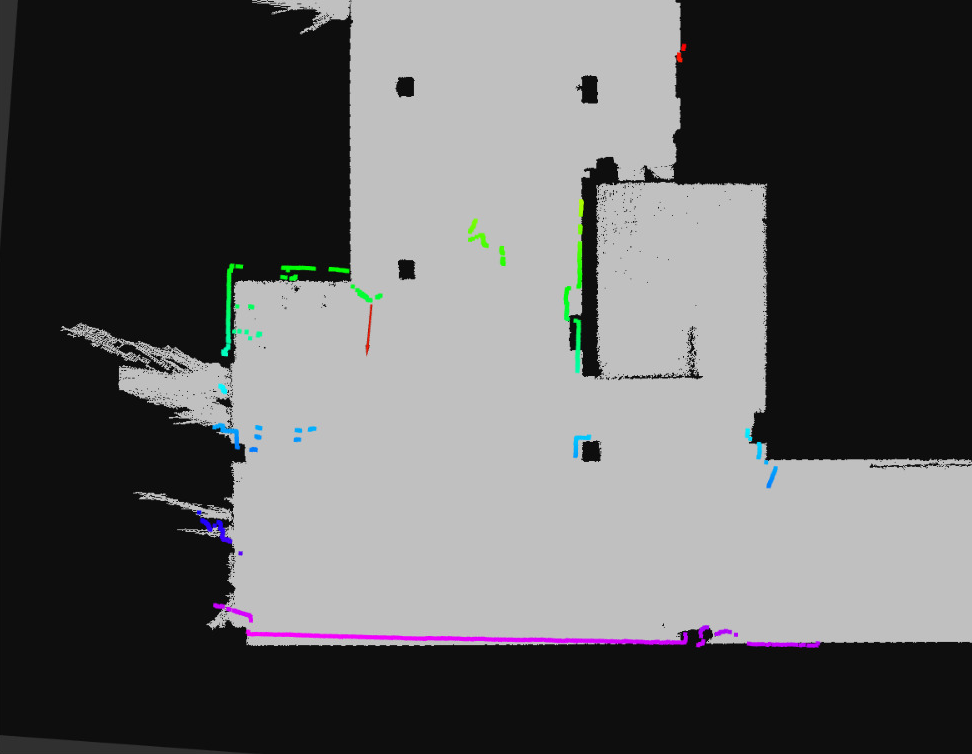
\includegraphics[width=1\textwidth]{figures/lidar_map.png}
  \caption{Dimostrazione funzionamento del sensore Lidar}
  \label{funzionamento_particle_filter}
\end{figure}

\noindent Figura \ref{funzionamento_particle_filter} llustra una breve dimostrazione del funzionamento del sensore Lidar. Nello specifico si riporta una porzione di mappa (grigia su sfondo nero) e la pointcloud generata dal sensore Lidar (punti colorati). Il colore dei punti non è casuale, ma è bensì un metodo intuitivo per mostrare graficamente la distanza di quel particolare punto dalla posizione calcolata del robot (freccia rossa).

\subsubsection{Planning}
\noindent La parte di planning si avvale di due nodi:

\begin{itemize}
  \item \textbf{path\_logger}: permette la registrazione di un percorso quando il veicolo viene guidato manualmente. Il percorso registrato viene poi salvato in un file apposito.
  \item \textbf{path\_publisher}: questo nodo si occupa di pubblicare un percorso preregistrato o precalcolato da seguire, pubblicato sul topic \textit{/path}.  
\end{itemize}

\subsubsection{Control}
\noindent Si passa infine a descrivere il funzionamento della parte di controllo, composta anch'essa da due nodi:

\begin{itemize}
  \item \textbf{purepursuit}: si occupa di ricevere il percorso pubblicato sul topic \textit{/path} e, a partire dalla posizione pubblicata dal nodo \textbf{particle\_filter}, di calcolare i comandi da impartire al veicolo. I comandi vengono pubblicati sul topic \textit{/drive\_parameters} e sono di tipo \textit{Ackermann Stamped}, un tipo di messaggio ROS che incapsula il timestamp, l'angolo di sterzo e la velocità desiderata
  \item \textbf{hunter\_ros2\_node}: come descritto in precedenza, questo nodo, oltre a fornire l'odometria del mezzo, è anche capace di ricevere i comandi da impartire al veicolo. Il nodo è infatti in perenne ascolto sul topic \textit{/drive\_parameters} e ad ogni messaggio comunicherà con l'interfaccia CAN del veicolo impartendogli la velocità e l'angolo di sterzo desiderati
\end{itemize}

\noindent Di seguito uno schema riassuntivo del funzionamento della guida autonoma:
\begin{figure}[h]
  \centering
  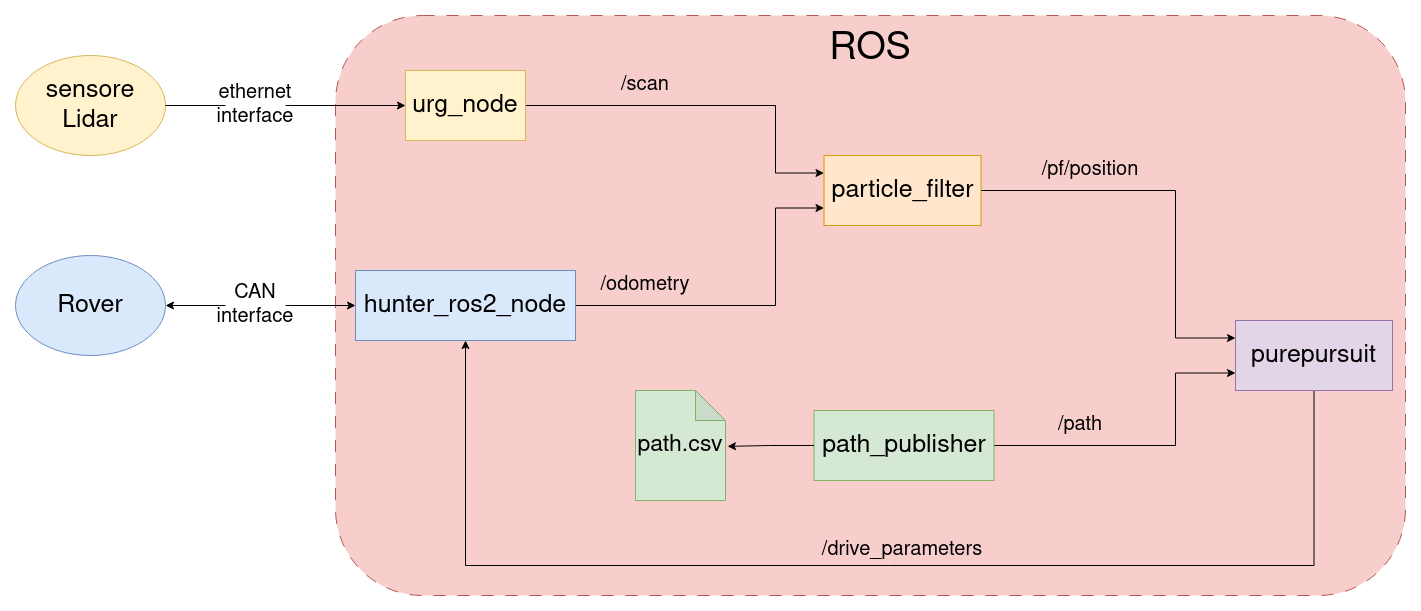
\includegraphics[width=1\textwidth]{figures/schema_guida_autonoma.png}
  \caption{Schema rissuntivo dello stack di guida autonoma}
  \label{Schema rissuntivo dello stack di guida autonoma}
\end{figure}

\subsection{Guida remota}
Una volta illustrato e compreso il funzionamento dello stack di guida autonoma, si passa alla descrizione di quella remota.

\noindent La prima scelta tecnica è stata quella di decidere quale parte dello stack spostare in remoto. Per esempio, si potrebbe decidere di svolgere solo la parte di planning da remoto e lasciare in resto in locale, o diversamente, portare sin remoto solo la perception. Si potrebbe anche decidere di far eseguire solo specifici nodi da remoto e lasciare in resto in locale.

\noindent Nella presente tesi si è scelto di portare in remoto quasi tutto lo stack, lasciando in locale solo i nodi che hanno strettamente bisogno dell'interfacciamento con l'hardware.

\noindent Nello specifico, gli unici nodi che rimarranno in locale saranno:

\begin{itemize}
  \item \textbf{urg\_node}: che sarà necessario per ricavare i dati dal sensore Lidar
  \item \textbf{hunter\_ros2\_node}: necessario per ricavare l'odometria del mezzo e per inviare i comandi all'interfaccia CAN
\end{itemize}

\noindent Tutto il resto sarà gestito da remoto. Questo permette di poter scegliere con più flessibilità in quale modo pilotare il rover. Si potrà infatti decidere sia di eseguire l'intero stack, senza modifiche, sulla macchina in remoto e di conseguenza inviare i comandi calcolati al mezzo, sia di poter guidare il veicolo completamente in manuale da un apposito operatore e di inviare solo i comandi scelti da quest'ultimo al veicolo.

\noindent Di seguito uno schema riassuntivo del funzionamento della guida remota:

\begin{figure}[h]
  \centering
  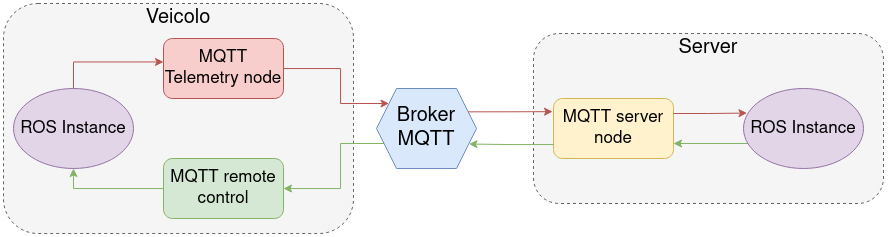
\includegraphics[width=1\textwidth]{figures/schema_guida_remota.png}
  \caption{Schema rissuntivo dello stack di guida remota}
  \label{Schema rissuntivo dello stack di guida remota}
\end{figure}

\subsection{Nodi sviluppati}
Oltre ai nodi già compresi nello stack di guida autonoma, è stato necessario sviluppare i nodi che permettessero lo scambio di informazioni tra il veicolo e il server. Nello specifico, i 3 nodi sono:
\begin{itemize}
    \item \textbf{mqtt\_telemetry\_node}: ha il compito di inviare i dati dei sensori dal veicolo al server
    \item \textbf{mqtt\_control\_node}: ha il compito di ricevere i dati di controllo dal server per poi pubblicarli su ROS
    \item \textbf{mqtt\_server\_node}: eseguito sul server, avrà il compito di ricevere sia i dati di telemetria da MQTT per poi ripubblicarli su ROS che ricevere i dati di controllo da ROS per poi ripubblicarli su MQTT
\end{itemize}

\noindent Ogni nodo è diviso in più classi ed un unico main file, che gestirà l'intero flusso di esecuzione del nodo. All'interno del progetto che contiene il nodo sono anche compresi dei file di configurazione in formato yaml, dai quali il nodo andrà a leggere informazioni necessarie per l'esecuzione del processo. Di seguito un esempio di file di configurazione utilizzato per definire alcuni parametri relativi alla comunicazione MQTT.

\lstinputlisting{samples/mqtt_parameters.yaml}

\noindent È inoltre utile specificare che l'intera codebase è scritta in linguaggio C++, che risulta utile qualora sia necessario avere bassi tempi di esecuzione.

\subsubsection{MQTT telemery node} \label{mqtt_telemetry_node}
La prima fase del progetto ha riguardato lo sviluppo di un componente software, ovvero un nodo ROS, in grado di interfacciarsi con i sensori del veicolo. Questo nodo, una volta configurato per sottoscriversi ai topic di interesse, è in grado di acquisire i dati provenienti dai sensori e di trasformarli in un formato adatto alla trasmissione. La scelta del formato JSON, ampiamente utilizzato per lo scambio di dati tra sistemi eterogenei, è stata dettata dalla sua leggibilità e dalla sua facilità di parsing. I dati, una volta formattati, vengono inviati al server MQTT.

\noindent I topic a cui il nodo effettua una subscribe sono:

\begin{itemize}
  \item \textit{/scan}: per la ricezione della pointcloud rilevata dal sensore Lidar
  \item \textit{/odometry}: per la ricezione dei dati di odometria del mezzo
\end{itemize}

\noindent Una volta acquisito il dato grezzo, esso viene convertito in una rappresentazione strutturata e leggibile, che nello specifico si compone di una stringa in formato JSON. Tale stringa, contenente l'insieme completo dei dati costituenti il messaggio, viene quindi immessa all'interno di una cache dedicata.

\noindent La cache funge da deposito temporaneo, accumulando le stringhe JSON generate fino al raggiungimento di una determinata soglia (o intervallo) di tempo predefinito e impostabile tramite file di configurazione. Al verificarsi di tali condizioni, il contenuto completo della cache viene trasmesso in un'unica operazione al server MQTT. Questa modalità di trasmissione, basata su un meccanismo di invio periodico, consente di ottimizzare le comunicazioni e ridurre il carico sulla rete.

\noindent Per quanto concerne la gestione concorrente di queste operazioni, si introduce il concetto di thread. Un thread può essere definito come un flusso di esecuzione autonomo all'interno di un processo. In altre parole, rappresenta una singola sequenza di istruzioni che può essere eseguita in parallelo rispetto ad altre sequenze, all'interno dello stesso programma.

\noindent Nel contesto descritto, è possibile impiegare un thread dedicato per gestire l'operazione di trasmissione dei dati. Tale thread opererà in modo concorrente rispetto al thread principale (main thread) consentendo di eseguire contemporaneamente altre attività e di migliorare la reattività dell'applicazione. Per fare questo è però necessario gestire la cache in modo che i 2 thread che ne fanno utilizzo non vadano in conflitto per accedere alla risorsa in quanto, se ciò non fosse gestito, si andrebbe ad incappare in problemi come, ad esempio, la lettura di un dato incorretto da parte del thread di invio dei messaggi o una scrittura parziale da parte del main thread.

\noindent Per la gestione di questi eventi si è dunque deciso di utilizzare una struttura chiamata mutex, che permette ad un thread di bloccare una risorsa per utilizzarla ed ad un altro di aspettare che la risorsa si liberi per poterla utilizzare. Di seguito l'implementazione della classe \textbf{msgs\_cache}:

\lstinputlisting{samples/msgs_cache.cpp}

\noindent Il nodo è suddiviso in 6 classi:

\begin{itemize}
  \item \textbf{conf\_loader}: si occupa di caricare i dati dai file di configurazione prima citati. Nello specifico, questa classe è stata implementata per rendere il main thread e il resto del processo indipendente dal formato dei file di configurazione
  \item \textbf{mqtt\_publisher}: è una classe che contiene metodi utili all'invio di stringhe tramite protocollo MQTT, avvalendosi della libreria paho.mqtt.cpp fornita dalla eclipse foundation 
  \item \textbf{mqtt\_telemetry\_node}: questa classe è quella che implementa il nodo ROS che si incaricherà di ricevere i dati utili alla telemetria
  \item \textbf{msgs\_cache}: questa classe implementa una semplice struttura dati che accoppia ad ogni topic ROS (rappresentata come stringa), una stringa JSON contente i dati di telemetria da inviare
  \item \textbf{msgs\_to\_string}: è un insieme di funzioni statiche che permette la traduzione da messaggi ROS a stringhe JSON
  \item \textbf{topic\_manager}: è la classe designata ad accoppiare i topic ROS con i rispettivi topic MQTT, il cui codice è incluso nella sezione \ref{gestione_dei_topic} 
\end{itemize}

\subsubsection{MQTT remote control} \label{mqtt_remote_control}
Successivamente, è fondamentale predisporre un meccanismo che consenta al veicolo di ricevere i comandi di controllo. A tal fine, è stato implementato un nodo dedicato che si sottoscrive al topic MQTT specificamente designato per la trasmissione di tali dati. Successivamente, il nodo ripubblica le informazioni ricevute sul topic ROS \textit{/drive\_parameters}.

\noindent Poiché i dati trasmessi tramite MQTT sono di tipo stringa, il veicolo dovrà elaborare queste stringhe al fine di estrarre le informazioni pertinenti e popolarne i campi di un messaggio ROS conforme al tipo di dato previsto, esattamente come descritto nella sezione 4.3.

\noindent il nodo in questo caso è suddiviso in 4 classi: 

\begin{itemize}
  \item \textbf{conf\_loader}: il cui funzionamento è riportato nella sezione \ref{mqtt_telemetry_node}
  \item \textbf{control\_node}: è il nodo incaricato di ripubblicare sul topic giusto i dati relativi al controllo
  \item \textbf{json\_to\_ros2\_msgs}: è il nodo incaricato alla conversione dei messaggi
  \item \textbf{mqtt\_subscriber}: è il nodo che si occupa alla sottoscrizione al topic mqtt designato alla ricezione dei dati
\end{itemize}

\noindent In questo caso non è stato necessario l'utilizzo della classe \textbf{topic\_manager} in quanto gli unici due topic in gioco (quello ROS e quello MQTT) sono entrambe impostabili da file di configurazione yaml.

\subsubsection{MQTT server node}
È stato infine implementato un nodo centrale, eseguito sul server, che funge da ponte di comunicazione tra il veicolo e l'istanza ROS del server stesso. Questo nodo è responsabile della ricezione di tutti i dati trasmessi dal veicolo tramite il protocollo MQTT e della loro successiva pubblicazione sul bus ROS. Contestualmente, il nodo si occupa di raccogliere i comandi di controllo generati all'interno dell'ambiente ROS, di incapsularli in un messaggio MQTT e di inoltrarlo al veicolo.

\noindent Il nodo in questo caso è suddiviso in 8 classi, alcune delle quali sono prese dai due nodi prima implementati:

%COSÌ FA CAFARE. SCRIVI ALMENO CHE TALE CLASSE È DESCRITTA IN TAL CAPITOLO, NON LASCIARE L'ELECON VUOTO
\begin{itemize}
  \item \textbf{conf\_loader}: il cui compito è riportato nella sezione \ref{mqtt_telemetry_node}
  \item \textbf{mqtt\_publisher}: il cui compito è riportato nella sezione \ref{mqtt_telemetry_node}
  \item \textbf{mqtt\_subscriber}: descritto nella sezione \ref{mqtt_remote_control}
  \item \textbf{msgs\_cache}: anch'esso descritto alla sezione \ref{mqtt_telemetry_node}
  \item \textbf{msgs\_to\_string}: riportato alla sezione \ref{mqtt_telemetry_node}
  \item \textbf{ros\_server\_node}: implementa il client ROS che andrà poi ad iscriversi e a pubblicare sui topic necessari
  \item \textbf{string\_to\_msgs}: al contrario di \textbf{msgs\_to\_string}, questa classe è incaricata di convertire le stringhe in formato JSON in messaggi ROS
  \item \textbf{topic\_manager}: già riportato alla sezione \ref{mqtt_telemetry_node}
\end{itemize}

\subsection{Gestione dei topic} \label{gestione_dei_topic}
Come descritto nella sezione \ref{mqtt_topic}, i topic ROS utilizzati hanno una struttura sostanzialmente diversa da quelli MQTT. Ai fini del progetto è stata dunque sviluppata una classe chiamata \textit{topic\_manager} che semplifica la gestione di questi due tipi di dati. La classe comprende 4 semplici metodi, 2 che riguardano il get ed il set di topic ROS e 2 che riguardano il get e il set dei topic MQTT, ad ogni topic MQTT è associato uno ROS e viceversa, di seguito i 4 metodi:

\lstinputlisting{samples/topic_manager.cpp}
\newpage
\section{Sviluppi futuri e conclusioni}
Per concludere, si va ad analizzare quali complicazioni sono state riscontrate durante lo sviluppo, quali falle rimangono ed eventuali soluzioni e sviluppi futuri e applicazioni pratiche della tesi.

\subsection{Problemi ed eventuali soluzioni}
Il primo dubbio riguardo il progetto descritto in questa tesi è sicuramente quello della latenza di rete: Applicazioni come quella della guida autonoma vengono chiamate real time, ciò vuol dire che l'esecuzione di ogni singolo pezzo dello stack deve eseguire in tempi stretti e che anche nel caso peggiore l'esecuzione non può superare una certa quantità di tempo, questa quantità viene chiamata deadline.  

\noindent È quindi spontaneo porsi un dubbio, ovvero quanto l'utilizzo della rete complichi il dover far rispettare le tempistiche. Includere la rete in applicazioni real time infatti diventa rischioso, si pensa subito al caso in cui la connessione sia molto scarsa o addirittur assente, quali complicazioni questo può portare. Anche nel caso di una situazione ottimale però bisogna sempre considerare quanto l'inclusione di un protocollo di rete (sepur leggero come nel caso di MQTT) porti dell'overhead e di conseguenza delle latenze nell'esecuzione.

\noindent possiamo ovviare a questi problemi (seppur limitatamente) grazie al meccanismo dei livelli di Quality Of Service che il protcollo ci fornisce, un livello basso di Quality Of Service infatti farà fare meno controlli al protocollo e di conseguenza rimuoverà un certo overhead. Anche la scelta del protocollo a livello transport influenza le latenze, se usare quindi UDP o TCP dato che notoriamente il protocollo UDP riduce di molto la complessità, a scapito però sempre della qualità del servizio.

\subsection{Sviluppi futuri}
Il progetto ai fini della tesi può considerarsi concluso, rimangono però eventuali implementazioni e test che potranno essere integrati in futuro.

\noindent La prima cosa che viene in mente è l'implementazione di uno stack di sicurezza informatica che permetta l'invio dei dati del mezzo su rete pubblica completamente criptati ed oscurati ad un possibile attaccante, implementazione necessaria se si prevede di utilizzare wurdts tecnologia in casi reali.

\noindent Un'ulteriore sviluppo possibile è l'aggiunta di una di una videocamera a bordo del mezzo, con la conseguente modifica del nodo di telemetria perchè possa inviare immagini della suddetta. Questo può essere utile al fine di permettere ad un operatore che si avvale della guida remota per potere vedere l'ambiente circostante in maniera più chiara rispetto che al singolo sensore Lidar.

\noindent Altro aspetto da considerare sarà l'implementazione di un sistema di platooning, per permettere al  server di poter guidare oltre che un unico mezzo anche una flotta, questo può rivelarsi molto vantaggioso se si prevede l'utilizzo di questa tecnologia , ad esempio, per il trasporto di merci.

\noindent Infine sarà necessario svolgere test in condizioni reali, condizioni in cui l'affidabilità alla rete sia limità o con ambienti molto complessi.

\subsection{Applicazioni pratiche}
Per concludere si procede ad elencare quali possono essere delle eventuali applicazioni pratiche di questa tecnologia.

\noindent Come descritto prima, un utilizzo potrebbe essere quello della creazione di una flotta di veicoli semi-autonomi connessi a scopi di trasporto, avere una flotta infatti di rover capaci di trasportare all'interno di ambienti lavorativi grandi quantità di materiale o semi-lavorati, aiuterebbe con lo sviluppo tecnologico di un'impresa.

\noindent Altro utilizzo pratico si può avere nel caso di veicoli ad utilizzo personale. Si può infatti ipotizzare uno scenario in cui il guidatore non sia in grado di controllare il veicolo in caso di emergena medica e che quindi si avvalga ad un servizio che preveda un operatore pronto a connettersi che possa pilotare il mezzo a distanza, o addirittura ad un servizio di guida autonoma che possa guidare il veicolo fino all'ospedale più vicino. 


\end{document}
